\documentclass[tikz,border=4pt]{standalone}
\usepackage{pgfplots}
\pgfplotsset{compat=1.16}
\pgfplotsset{
  bode/.style={
    width=6.4cm, height=4.4cm, xmin=0.01, xmax=100,
    grid=both, major grid style={gray!55}, minor grid style={gray!20},
    tick label style={font=\footnotesize}, label style={font=\small},
    title style={font=\small}, xlabel={$\omega/\omega_u$},
  },
  bode mag/.style={bode, ymin=-50, ymax=50, ytick={-40,-20,0,20,40},
    ylabel={$|H|_{\mathrm{dB}}$}, title={Modulo}},
  bode fase/.style={bode, ymin=-100, ymax=100, ytick={-90,-45,0,45,90},
    ylabel={$\varphi$ [$^\circ$]}, title={Fase}},
}
\begin{document}
% Derivatore con perdita: H(j w) = -j w R2 C / (1 + j w/wc),  wc = 1/(R1 C)
% R1 in serie al condensatore d'ingresso, R2 in retroazione.
% Esempio della lezione: R2/R1 = 10  ->  wu = 1/(R2 C),  wc = 10 wu.   x = w/wc
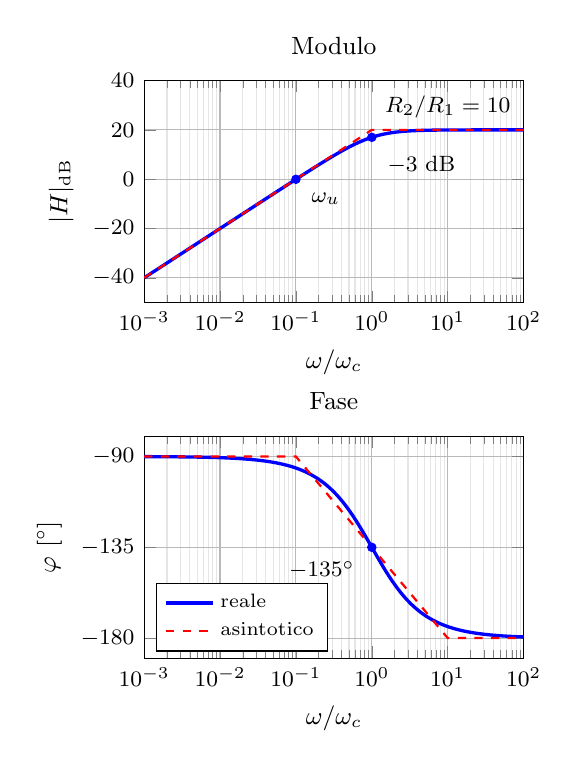
\begin{tikzpicture}
% ---------- modulo ----------
\begin{semilogxaxis}[bode mag, name=mag, xmin=0.001, xmax=100, xlabel={$\omega/\omega_c$},
  ymin=-50, ymax=40, ytick={-40,-20,0,20,40}]
  \addplot[blue, very thick, domain=-3:2, samples=201] ({10^x}, {20+20*x-10*log10(1+10^(2*x))});
  % asintotico: +20 dB/dec fino a wc, poi piatto a 20 log(R2/R1)
  \addplot[red, thick, dashed] coordinates {(0.001,-40) (1,20) (100,20)};
  \addplot[only marks, mark=*, mark size=1.5pt, blue] coordinates {(1,16.99) (0.1,-0.04)};
  \node[anchor=south east, font=\footnotesize] at (axis cs:90,21) {$R_2/R_1=10$};
  \node[anchor=north west, font=\footnotesize] at (axis cs:1.2,13.5) {$-3$ dB};
  \node[anchor=north west, font=\footnotesize] at (axis cs:0.12,-1.5) {$\omega_u$};
\end{semilogxaxis}
% ---------- fase ----------
\begin{semilogxaxis}[bode fase, at={(mag.south west)}, yshift=-1.7cm, anchor=north west,
  xmin=0.001, xmax=100, xlabel={$\omega/\omega_c$},
  ymin=-190, ymax=-80, ytick={-180,-135,-90},
  legend style={font=\scriptsize, at={(0.03,0.03)}, anchor=south west},
  legend cell align=left]
  \addplot[blue, very thick, domain=-3:2, samples=201] ({10^x}, {-90-atan(10^x)});
  % asintotico: -90 fino a wc/10, rampa di -45 gradi/dec, -180 da 10 wc
  \addplot[red, thick, dashed] coordinates {(0.001,-90) (0.1,-90) (10,-180) (100,-180)};
  \legend{reale, asintotico}
  \addplot[only marks, mark=*, mark size=1.5pt, blue, forget plot] coordinates {(1,-135)};
  \node[anchor=north east, font=\footnotesize] at (axis cs:0.8,-137) {$-135^\circ$};
\end{semilogxaxis}
\end{tikzpicture}
\end{document}